\documentclass[xetex, onlymath]{beamer}
\usefonttheme{serif}
\usetheme{hsr}

% select font
\usepackage[T1]{fontenc}
\usepackage[usefilenames]{plex-otf}
\renewcommand*\familydefault{\sfdefault}

\usepackage{booktabs}
\usepackage{array}

% pretty drawings
\usepackage{tikz}
\usetikzlibrary{%
    decorations.pathreplacing,%
    decorations.pathmorphing%
}

\usepackage{pgfplots}
\pgfplotsset{compat=1.15}

\usepackage{listings}
%% create a lstlisting style
\lstdefinestyle{samplestyle}{
    belowcaptionskip=\baselineskip,
    breaklines=true,
    frame=none,
    inputencoding=utf8,
    % margin
    xleftmargin=\parindent,
    % numbers
    numbers=left,
    numbersep=5pt,
    numberstyle=\ttfamily\footnotesize\color{hsr-black40},
    % background
    backgroundcolor=\color{hsr-lightgrey20},
    % default language:
    language=[LaTeX]TeX,
    showstringspaces=false,
    % font
    basicstyle=\ttfamily\small,
    identifierstyle=\color{hsr-black},
    keywordstyle=\color{hsr-blue},
    commentstyle=\color{hsr-black40},
    stringstyle=\color{hsr-mauve80},
}

%% and set the chosen style
\lstset{style=samplestyle, escapechar=`}


% metadata
\title{\textrm{\LaTeX} Workshop}
\author[NaoPross]{Naoki Pross \texttt{<npross@hsr.ch>}}
\date{\today}

\institute[HSR]{Hochschule f\"ur Technik Rapperswil}
%\logo{
\includegraphics[width=3cm]{figs/hsr-logo}}

\AtBeginSection[]
{
  \begin{frame}
    \frametitle{Table of Contents}
    \tableofcontents[currentsection]
  \end{frame}
}


\begin{document}
\begin{frame}
\maketitle
\end{frame}

\begin{frame}{Why \textrm{\LaTeX}}
	\begin{center}
		\begin{tikzpicture}
			\begin{axis}[
				smooth, samples = 100,
				axis lines = left,
				axis line style = { thick },
				width = \textwidth,
				height = \axisdefaultheight,
				grid style = dashed,
				xlabel = Complexity,
				ylabel = Difficulty,
				x label style={at={(axis description cs:1,.1)},anchor=east},
				ytick = \empty,
				xtick = {2, 4, 6, 11, 13, 16, 20, 22},
				xticklabels = {Text, Figures, Tables, Math, Plots, Diagrams, Thesis, Book},
				x tick label style = { rotate = 80, anchor = east, font=\footnotesize },
				legend style = { legend pos = north west },
				no markers, domain = 0:25,
			]
				\plot[very thick, hsr-mauve60, domain=0:14]{exp(x/3 - 2.5)};
				\addlegendentry{Word}
				\plot[very thick, hsr-blue]{3/(1 + exp(-2*(x-2.5))) + x/50*exp((x-4)/12)};
				\addlegendentry{\textrm{\LaTeX}}
			\end{axis}
		\end{tikzpicture}
	\end{center}
\end{frame}

\begin{frame}{Goal: Learn to typeset something like this}
	\begin{center}
		\vspace{1cm}
		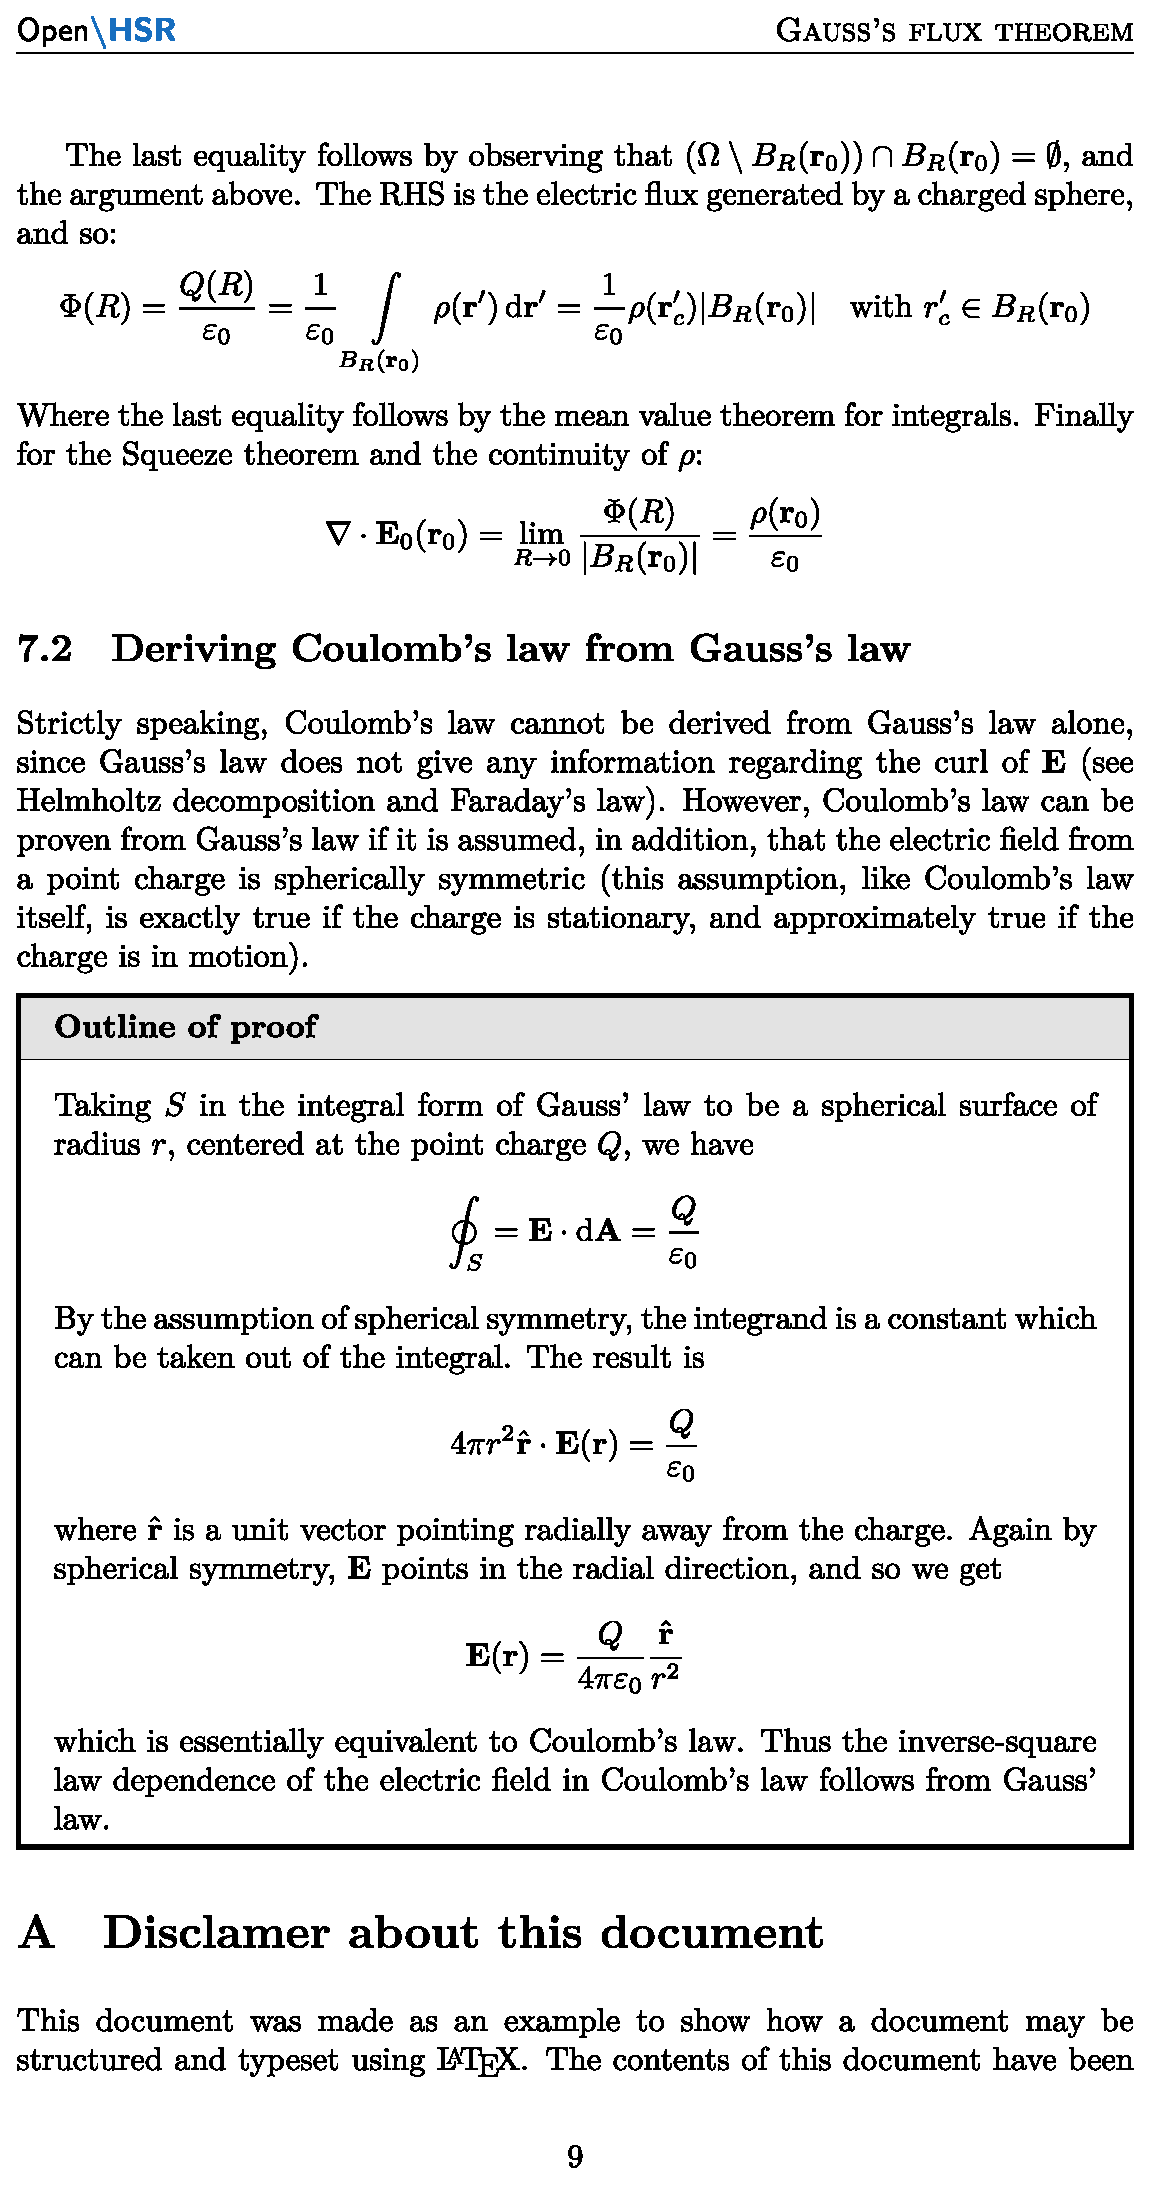
\includegraphics[width=.8\linewidth]{figs/gauss-flux}
	\end{center}
\end{frame}

\section{Introduction}

\begin{frame}{What is Typesetting}
\end{frame}

\begin{frame}{History \& \textrm{\LaTeX}}
\end{frame}

\section{Fundamentals}
\begin{frame}{Source code spacing}
\end{frame}

\begin{frame}{Special characters}
\end{frame}

\begin{frame}{Commands}
\end{frame}

\begin{frame}{Environments}
\end{frame}

\begin{frame}{Document structure}
\end{frame}

\begin{frame}{Spacing and newlines}
\end{frame}

\section{Basics}
\begin{frame}[fragile]{Emphasis, Bold, Italic, \ldots}
\begin{lstlisting}
This is \emph{emphatized}.
You may also use
\textbf{Bold},
\textit{Italic},
\textsf{Sans-Serif},
\textsc{SmallCaps},
\textrm{Roman},      % with serif
\texttt{Typewriter}. % monospaced
\end{lstlisting}

\begin{exampleblock}{}
This is \emph{emphatized}.
You may also use
\textbf{Bold},
\textit{Italic},
\textsf{Sans-Serif},
\textsc{SmallCaps}\footnote{The font used in this presentation does not have smallcaps shapes},
\textrm{Roman} or
\texttt{Typewriter}.
\end{exampleblock}
\end{frame}

\begin{frame}[fragile]{Lists}
\begin{columns}
\begin{column}{.5\linewidth}
\begin{lstlisting}
\begin{itemize}
  \item Tomatoes
  \item Peppers
  \item Broccoli
\end{itemize}
\end{lstlisting}

\begin{lstlisting}
\begin{enumerate}
  \item Discovery coffee
  \item Get addicted
  \item Congratulations
\end{enumerate}
\end{lstlisting}
\end{column}

\begin{column}{.4\linewidth}
\begin{exampleblock}{Itemize}
	\begin{itemize}
		\item Tomatoes
		\item Peppers
		\item Broccoli
	\end{itemize}
\end{exampleblock}
\begin{exampleblock}{Enumerate}
	\begin{enumerate}
		\item Discovery coffee
		\item Get addicted
		\item Congratulations
	\end{enumerate}
\end{exampleblock}
\end{column}
\end{columns}
\end{frame}

\begin{frame}[fragile]{Description}
\begin{lstlisting}
\begin{description}
  \item[Programmer] A person who is paid to professionally scream at a computer.
  \item[Manager] A person who appears to know how all tasks should be accomplished but can't actually do any of those tasks themselves.
\end{description}
\end{lstlisting}

\begin{exampleblock}{}
\begin{description}
  \item[Programmer] A person who is paid to professionally scream at a computer.
  \item[Manager] A person who appears to know how all tasks should be accomplished but can't actually do any of those tasks themselves.
\end{description}
\end{exampleblock}
\end{frame}

\begin{frame}{Floating elements}
\begin{table}
	\caption{Floats placing permissions}
	\begin{tabular}{>{\ttfamily}l l}
		\toprule
		\textsf{Specifier} & Permission \\
		\midrule
		h & Place around here \\
		t & At the top of the page \\
		b & At the bottom of the page \\
		p & On a special page containing only floats \\
		! & ``I don't care if it will be ugly'' \\
		H\footnote{Requires the ``\texttt{float}'' package, i.e. 
			``\texttt{\textbackslash usepackage\{float\}}''} 
		  & Place \textbf{exactly here} (may look very ugly) \\
		\bottomrule
	\end{tabular}
\end{table}
\end{frame}

\begin{frame}[fragile]{Tables and tabular}
\begin{lstlisting}
\begin{table}[h]
  \caption{Not up to date numbers}
  \begin{tabular}{l r r}
    `\textcolor{hsr-mauve}{\textbackslash toprule\textsuperscript{1}}`
    Country & Infected & Deaths \\
    `\textcolor{hsr-mauve}{\textbackslash midrule\textsuperscript{1}}`
    China       & 80'652 & 3'070 \\
    South Korea &  7'041 &    44 \\
    Italy       &  5'833 &   233 \\
    `\textcolor{hsr-mauve}{\textbackslash bottomrule\textsuperscript{1}}`
  \end{tabular}
\end{table}
\end{lstlisting}
\begin{alertblock}{\textsuperscript{1} Pro Tip}
	Add ``\texttt{\textbackslash usepackage\{booktabs\}}'' to use
	rulers.
\end{alertblock}
\end{frame}

\begin{frame}{Tables and tabular}
\begin{exampleblock}{}
\begin{table}
  \caption{Not up to date numbers}
  \begin{tabular}{l r r}
    \toprule
    Country & Infected & Deaths \\
    \midrule
    China       & 80'652 & 3'070 \\
    South Korea &  7'041 &    44 \\
    Italy\footnote{Congratulations, your public health worse than Iran's}
    &  5'833 &   233 \\
    \bottomrule
  \end{tabular}
\end{table}
\end{exampleblock}
\end{frame}


\begin{frame}{Figures}
\end{frame}

\begin{frame}[fragile]{Cross-References}
\begin{lstlisting}
\section{Introduction} 
... will be discussed in \S \ref{sec:nvstokes} ...

\section{Stokes equation} \label{sec:nvstokes}
\end{lstlisting}

\begin{exampleblock}{Document}
\textbf{1\; Introduction} \\[.2em]
\ldots{} will be discussed in \S 4 \ldots{}
\\[1em]

\textbf{4\; Stokes Equation} \\[.2em]
\ldots{}
\end{exampleblock}

\begin{alertblock}{Pro Tip}
Use prefixes such as \texttt{sec:}, \texttt{fig:}, \texttt{tab:} to avoid mistakes.
\end{alertblock}
\end{frame}

\begin{frame}[fragile]{Cross-References}
\begin{columns}
\begin{column}{.5\linewidth}
\begin{lstlisting}
\begin{figure} % or table
  \includegraphics{...}
  \caption{Reflection and refraction of electromagnetic waves.}
  \label{fig:refl}
\end{figure}

... as shown in figure
\ref{fig:refl} ...
\end{lstlisting}
\end{column}
\begin{column}{.5\linewidth}
\begin{exampleblock}{Figure reference}
\begin{figure}[h]
	\newsavebox\reflfigbox%
	\begin{lrbox}{\reflfigbox}%
		% Oblique Incidence with using basics instructions
% Author: Edgar Fuentes (Club de LaTeX UC member)
%
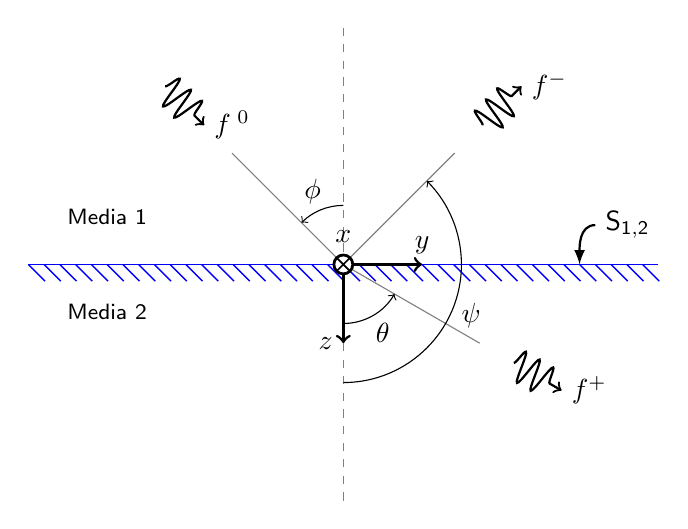
\begin{tikzpicture}[
    media/.style={font={\footnotesize\sffamily}},
    wave/.style={
        decorate,decoration={snake,post length=1.4mm,amplitude=2mm,
        segment length=2mm},thick},
    interface/.style={
        % The border decoration is a path replacing decorator. 
        % For the interface style we want to draw the original path.
        % The postaction option is therefore used to ensure that the
        % border decoration is drawn *after* the original path.
        postaction={draw,decorate,decoration={border,angle=-45,
                    amplitude=0.3cm,segment length=2mm}}},
    ]
    % Round rectangle
    \fill[white] (-4,-3) rectangle (4,0);
    % Interface
    \draw[blue,line width=.5pt,interface](-4,0)--(4,0);
    % Vertical dashed line
    \draw[dashed,gray](0,-3)--(0,3);
    % Coordinates system
    \draw(0,0.15)node[above]{$x$};
    \draw[<->,line width=1pt] (1,0) node[above]{$y$}-|(0,-1) node[left]{$z$};
    % Incidence
    \draw[->,wave]
         (135:3.2cm)--(135:2.5cm)node[right]{\(f^{\;0}\)};
    \draw[gray](0:0cm)--(135:2cm);
    \path (0,0)++(113:1cm)node{$\phi$};
    \draw[->](0,0.75)arc(90:135:.75cm);
    % Transmission
    \draw[->,wave]
         (-30:2.5cm)--(-30:3.2cm)node[right]{$f^+$};
    \draw[gray](0:0cm)--(-30:2cm);
    \path (0,0)++(-60:1cm)node{$\theta$};
    \draw[->] (0,-0.75) arc (-90:-30:.75cm);
    % Reflection
    \draw[->,wave]
         (45:2.5cm)--(45:3.2cm)node[right]{$f^-$};
    \path (0,0)++(-22:1.75cm) node{$\psi$};
    \draw[gray](0:0cm)--(45:2cm);
    \draw[->] (0,-1.5)arc(-90:45:1.5cm);
    % Media names
    \path[media] (-3,.6)  node {Media 1}
                 (-3,-.6) node {Media 2};

    % $x$ axis
    \filldraw[fill=white,line width=1pt](0,0)circle(.12cm);
    \draw[line width=.6pt] (0,0)
                          +(-135:.12cm) -- +(45:.12cm)
                          +(-45:.12cm) -- +(135:.12cm);
    % Interface pointer
    \draw[-latex,thick](3.2,0.5)node[right]{$\mathsf{S_{1,2}}$}
         to[out=180,in=90] (3,0);
    % To-paths are really useful for drawing curved lines. The above
    % to path is equal to:
    %
    % \draw[-latex,thick](3.2,0.5)node[right]{$\mathsf{S_{1,2}}$}
    %      ..controls +(180:.2cm) and +(up:0.25cm) .. (3,0);
    % Internally the to path is translated to a similar bezier curve,
    % but the to path syntax hides the complexity from the user. 
\end{tikzpicture}

	\end{lrbox}
	\resizebox{\textwidth}{!}{\usebox\reflfigbox}%
	\caption{Reflection and refraction of electromagnetic waves.}
	\label{fig:refract}
\end{figure}
\ldots{} as shown in figure \ref{fig:refract} \ldots{}
\end{exampleblock}
\end{column}
\end{columns}
\end{frame}

\section{Mathematics}
\begin{frame}{Math environments}
\end{frame}

\begin{frame}{Math symbols and fonts}
\end{frame}

\begin{frame}{Equations}
\end{frame}

\begin{frame}{Spacing in math mode}
\end{frame}

\section{Bibliography management}
\begin{frame}{TheBibliography}
\end{frame}

\begin{frame}{External bibliography}
\end{frame}

\section{Extras}
\begin{frame}{Source code listings}
\end{frame}

\begin{frame}{Plots}
\end{frame}

\begin{frame}{TikZ}
\end{frame}

\end{document}